\documentclass{article}
\usepackage{graphicx}% Required for inserting images
\usepackage{lindrew}
\usepackage[shortlabels]{enumitem}
\usepackage{pdfpages}
\usepackage{enumerate}
\usepackage{algorithm}
\usepackage{algpseudocode}
\usepackage{matlab-prettifier}
\usepackage{pythonhighlight}

\title{CS 156a Problem Set 8}
\author{Amitesh Pandey}
\date{November 2024}

\begin{document}
\maketitle
\section*{Primal versus Dual Problem}
\subsection*{Problem 1}
Recall that the formulation is
\begin{equation*}
    \text{min} \left(\frac{1}{2}\mathbf{w}^{T}\mathbf{w}\right)
\end{equation*}
subject to $y_{n}(\mathbf{w}^{T}x_{n} + b) \geq 1,  \forall n$. The components of $\mathbf{w}$ and the bias $b$ compose of all the variables in this problem. Thus it is a $d + 1$ variable quadratic programming problem. Option $\textbf{[d]}$ is correct.\\\\
\noindent{\textbf{Note: }} Code for all following problems is attached at the end.
\section*{Polynomial Kernels}
\subsection*{Problem 2}
We can see that with $E_{\text{in}} = 0.11$, $\textbf{[a]}$, 0 versus all, has the highest $E_{\text{in}}$. 
\subsection*{Problem 3}
We can see that with $E_{\text{in}} = 0.021$, $\textbf{[a]}$, 1 versus all, has the highest $E_{\text{in}}$. 
\subsection*{Problem 4}
We can see that 0 versus all has a vector size of 2179, whereas 1 versus all has a vector size of 386, so 2179 - 386 = 1793, which is closest to option $\textbf{[c]}$.
\subsection*{Problem 5}
We can see that the maximum $C = 1$ achieves the lowest $E_{\text{in}} = 0.0032$, so option $\textbf{[d]}$ is correct.
\subsection*{Problem 6}
At $C = 0.001$, $Q = 2$ has a support vector of size 76 and $Q = 5$ has a vector of size 25, so $\textbf{[b]}$ is correct.
\newpage
\section*{Cross Validation}
\subsection*{Problem 7}
Out of the $100 \times 10 = 1000$ folds, we can see that $C = 0.001$ was selected the most times, by having the lowest error 526 times. So $\textbf{[b]}$ is correct.
\subsection*{Problem 8}
We get the error for $C = 0.001$ as $0.0047$, closest to $0.005$ so $\textbf{[c]}$ is correct.
\section*{RBF Kernel}
\subsection*{Problem 9}
With $E_{\text{in}} = 0.006$, it was $C = 10^6$ that achieved the lowest $E_{\text{in}}$. So option $\textbf{[e]}$ is correct.
\subsection*{Problem 10}
With $E_{\text{out}} = 0.018$, it was $C = 100$ that achieved the lowest $E_{\text{out}}$. So option $\textbf{[c]}$ is correct.
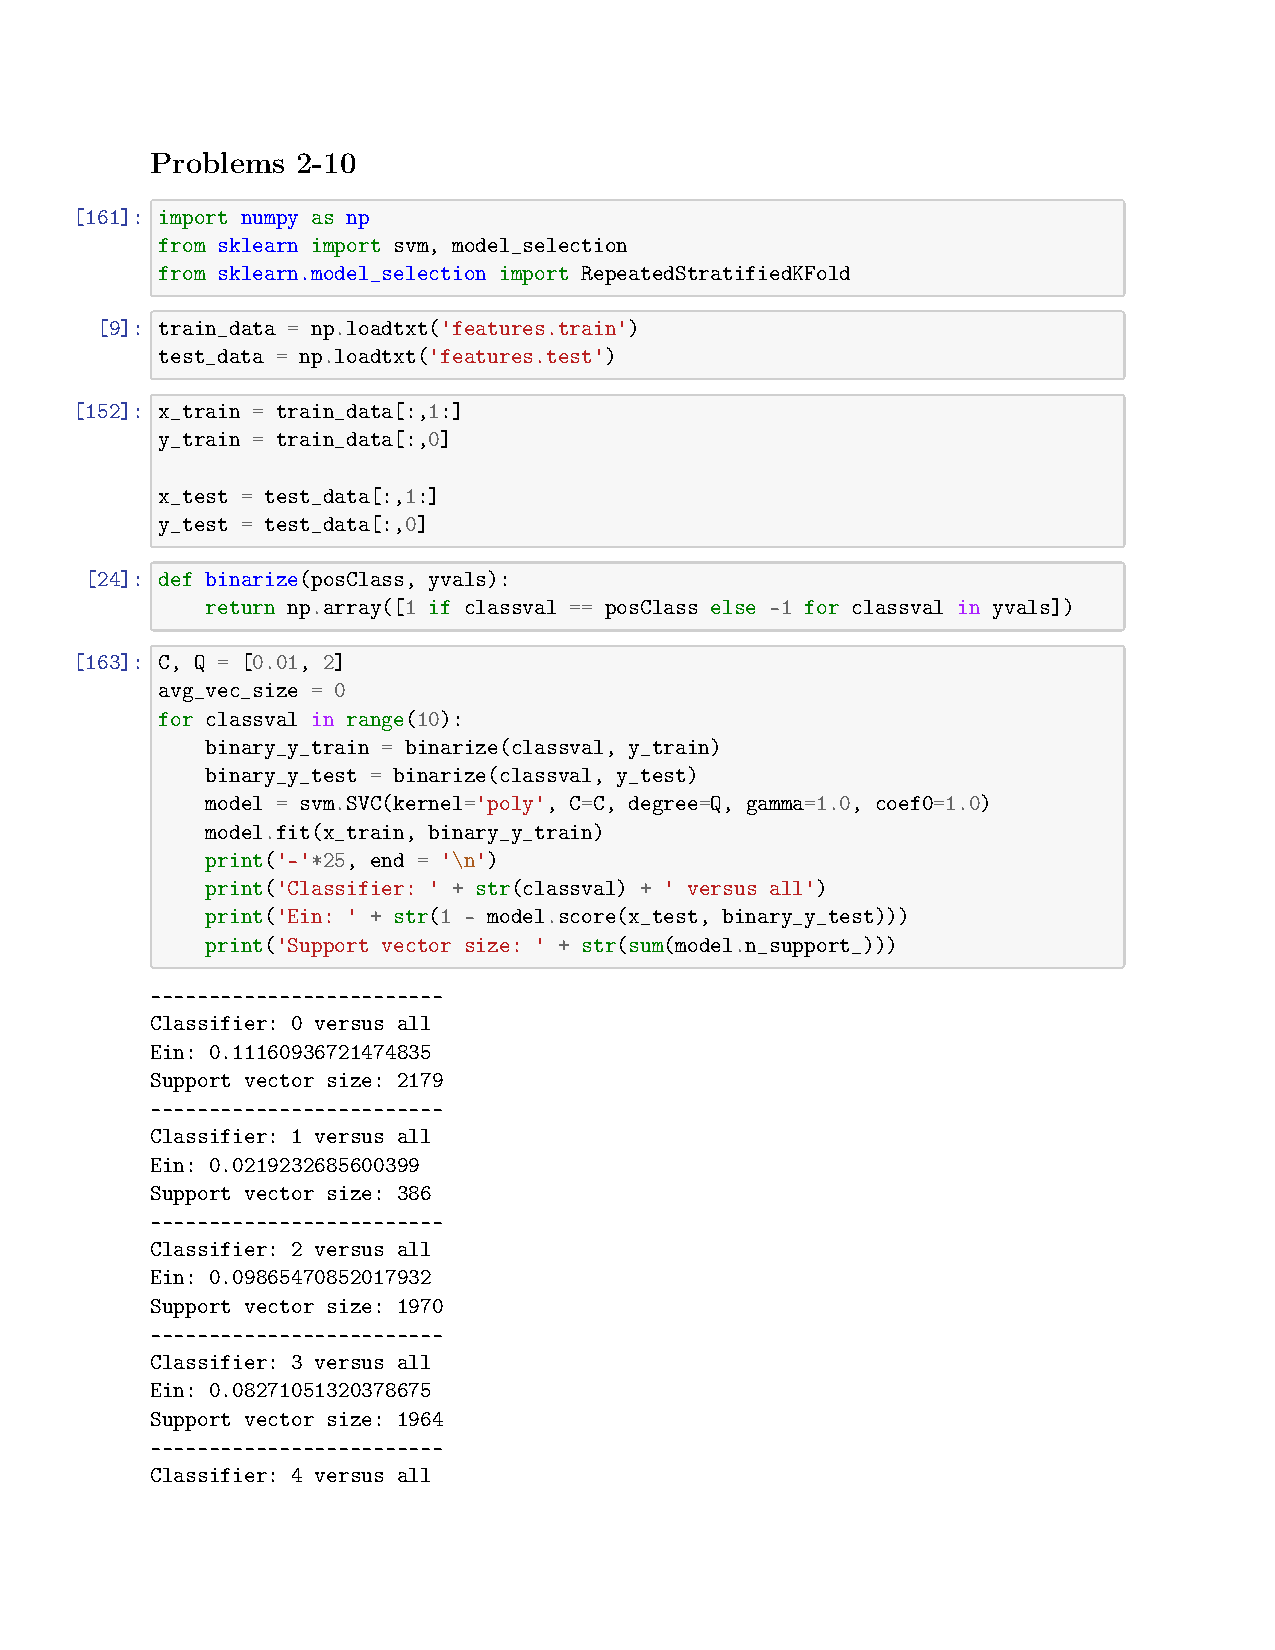
\includepdf[pages=-]{Code_for_HW8.pdf}
\end{document}
